%!TEX root = ../main.tex
\newcommand\independent{\protect\mathpalette{\protect\independenT}{\perp}}
\def\independenT#1#2{\mathrel{\rlap{$#1#2$}\mkern2mu{#1#2}}}

\section{Hierarchical Mixture of Experts [40 pts] (Xiongtao)}

\noindent
In this problem, we are going to work with a two-level hierarchical mixture of experts network (HME). Let
$\xv \in \Rb^{r}$ is the input, $\yv\in \Rb^{s}$ is the output. If $\yv$ is defined in a continuous space, it is a regression problem, and if $\yv$ is defined in categories, it is a classification problem. The dataset consists of $T$ paired observations $\Xc = \{(\xv^{(t)}, \yv^{(t)})\}$, where $t=1, ..., T$. Here we are going to use HME to work on regression problems.

The basic structure of an HME is shown in Figure \ref{fig:hme}. An HME is a tree in which non-terminals are gating networks and leaf nodes are expert networks. Both gating networks and expert networks use $\xv$ as input. Usually, expert networks and gating networks are modeled as generalized linear model (GLM). Expert networks consist of some simple models, i.e. linear regression (for regression), Bernoulli probability model (for classification) and so on. Each of them produces a variable $\muv_{ij}$ for each input vector. Gating networks consist of distributions that generate a partition of unity at each point in the input space, for example, they could be softmax operations on $\xv$. Intuitively, expert networks define the relationship between observation and response, while gating networks act as prior/weights for expert networks, determining which expert networks are going to make a decision about $\xv$. Because gating networks also depend on data, there would various combinations of expert networks used for decisions for different $(\xv, \yv)$. Therefore, HME can model complex data by the combination of some simple models. 
	
\begin{figure}[!ht]
	\centering
	% Requires \usepackage{graphicx}
	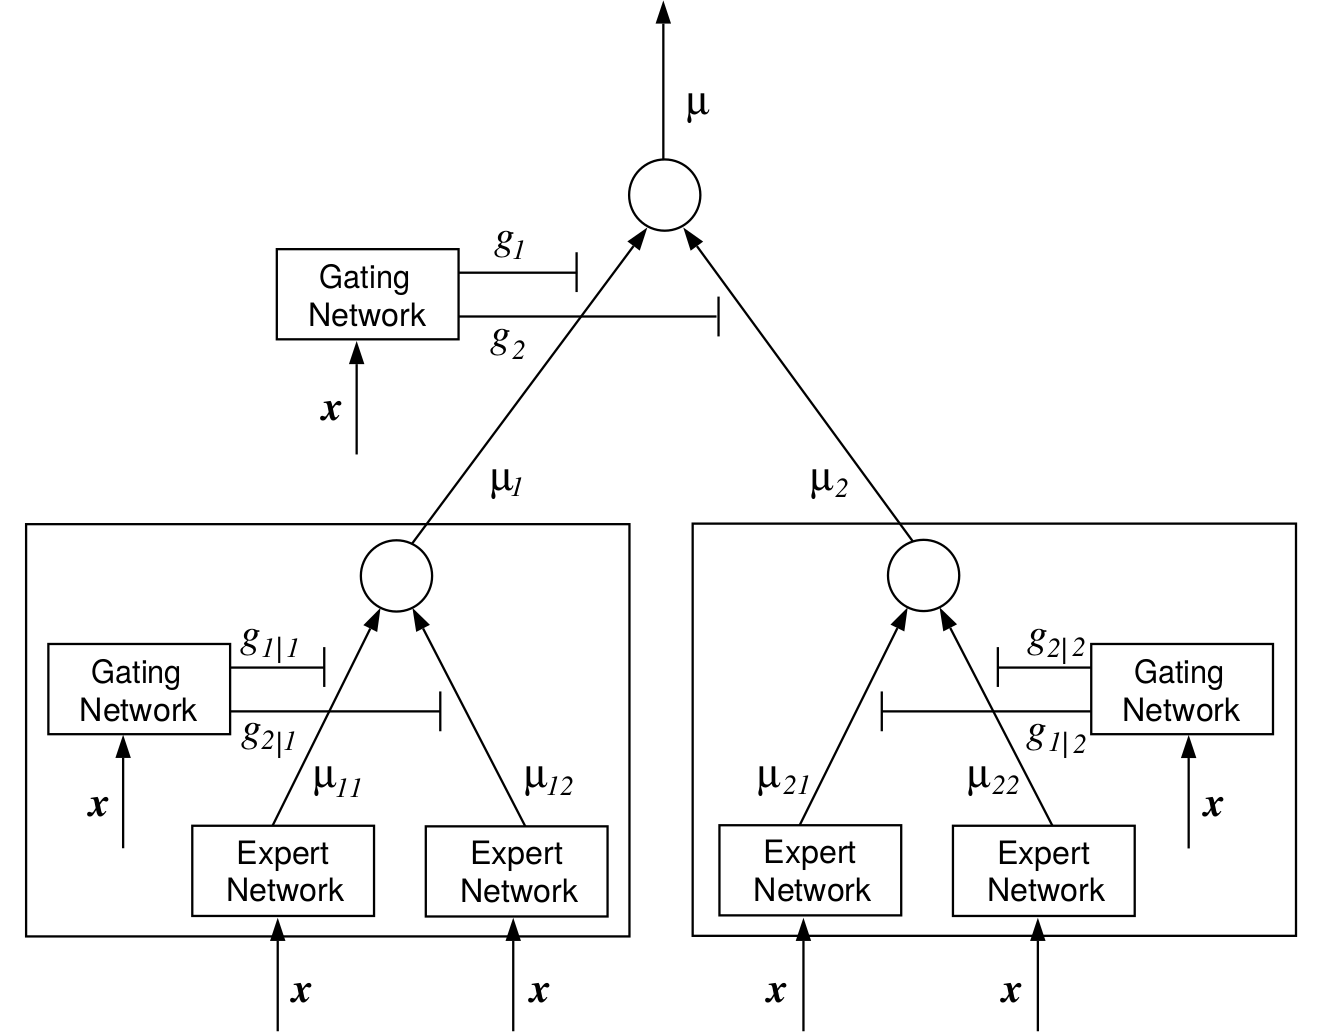
\includegraphics[width=0.6\textwidth]{figures/2_layer_HME.png}\\
	\caption{A two-level hierarchical mixture of experts.}
	\label{fig:hme}
\end{figure}


In the HME, there are $MN> 0$ expert networks in the bottom layer, we use $ENet_{ij}$ to represent expert networks with index $i, j$, $i=1:M$, $j=1:N$. All $ENet_{ij},~j=1:N$ are children of $i-th$ node in the middle layer of the tree. Here, the expert networks are defined as linear regression models, with 
$$\muv_{ij} \sim \Nc(\Uv_{ij}\xv, \sigma_{i}^2\Iv)$$
where $\sigma_i$ is shared among $i-th$ block of expert networks $ENet_{ij}\quad j=1,...,N$, $\Uv_{ij}$ is the weight matrix, and $\Iv$ is the identity matrix. 

For the gating network in the top level, it is a "softmax" function of $\vv_{i}\xv$ as
$$g_{i} = \frac{e^{\vv_{i}^T\xv}}{\sum_{i'}e^{\vv_{i'}^T\xv}}$$
where $\vv_{i}$ is a weight vector, $i=1:M$. Clearly, $g_i$ is a GLM for $\xv$. 

For gating network in the lower level, we also define them as a GLM of $\xv$, as

$$g_{j|i}(\xv) = \frac{e^{\vv_{ij}^T\xv}}{\sum_{k}e^{\vv_{ik}^T\xv}}$$
where $j=1:N$.  

As we mentioned before, gating networks could be viewed as weight of each node. Therefore, the output vector at each non-terminal node of the tree is the weighted output of the experts below that node, i.e. for $i-th$ node in the middle layer, the output is
$$\muv_i = \sum_j g_{j|i}\muv_{ij}$$
and the output at the top level is:
$$\muv = \sum_i g_i\muv_i$$


Finally, we define the response variable $\yv$ as a (conditional) linear regression on the output of each expert network $\muv_{ij}$ as 
$$P(\yv|\muv_{ij}, \sigma) = \Nc(\muv_{ij}, \sigma^2I)$$ 
Where $\sigma$ is the standard deviation, which is shared for the whole network. 

From another point of view, we treat the gating networks as prior for $\yv$ and the expert networks as conditional distribution with data, then we can get the distribution as
$$P(\yv, \muv|\xv, \thetav) = \sum_{i}g_i(\xv, \vv_{i})\sum_{j}g_{j|i}(\xv, \vv_{ij})P(\yv|\muv_{ij}, \sigma)P(\muv_{ij}|\xv, \sigma_{i})$$
where $\muv = \{\muv_{11}, ..., \muv_{MN}\}$, and $\thetav$ represents all parameters in the network, i.e. for both expert networks and gating networks.

We can also define a posterior probability associated with each node, that reflects the extent to which the node is activated. For the top level nodes, using the Bayes Rule, we define the posterior probabilities as 
$$h_{i} = \frac{g_{i}\sum_{j}g_{j|i}P_{ij}(\yv|\xv, \theta)}{\sum_{i}g_{i}\sum_{j}g_{j|i}P_{ij}(\yv|\xv, \theta)}$$
where $$P_{ij}(\yv|\xv, \thetav_E) \defeq \sum_{\muv_{ij}}P(\yv|\xv, \muv_{ij}, \sigma)P(\muv_{ij}|\xv, \sigma_{i})$$
which is the factorized distribution associated with each expert network, and $\thetav_E$ represents all parameters associated with expert networks, i.e. $\thetav_E = \{\sigma_i,~i=1:M\} \cup \{\sigma\}\cup\{\Uv_{ij},~~ i=1:M, ~~j=1:N \}$.

\subsection*{3.1. Warm up [2 + 1 + 1 = 4 pts]}

\begin{enumerate}
\item a problem in the model is that there are latent variables $\muv$ in the full distribution, which complicate the model. Therefore, we would like to marginalize out $\muv$ first. Please derive $p(\yv|\xv, \theta)$. You can keep $g_{i}$ and $g_{j|i}$ in the distribution, and just work with other parts of the distribution. In the later part of the question, we will just use the marginal distribution, therefore, please be careful and make sure your derivation is correct. 

Hint: Linear Gaussian system would be helpful here.

\item Write out the posterior distributions at the nodes in the bottom level of the network, that is, $h_{j|i}$. 

\item HME is considered as a nonlinear model for $\xv$ and $\yv$, reasoning why this network is a nonlinear model.  

\end{enumerate}


\subsection*{3.2. EM algorithm for HME [19 pts]}

To derive the EM algorithm, we first define binary latent variables $z_i$ and $z_{j|i}$ that associate with the nodes in the network. $z_{j|i}=1$ means expert network $ENet_{ij}$ is activated, $z_i=1$ means node $i$ in top layer is activated. For the bottom layer, we only allow one expert network for the children of $i-th$ node in the top layer being activated, that is $\sum_{j}z_{j|i} = 1$, and we also just allow one node in the top level activated, that is, $\sum_{i}z_i=1$. We define $z_{ij}= z_{i}z_{j|i}$, which could be interpreted as the activation of the specific expert network.

With $z_i$ and $z_{j|i}$, we could rewrite the distribution for a single data point as
$$P(\yv, \zv|\xv, \thetav) = \prod_{i}\prod_{j}(g_i g_{j|i}P_{ij}(\yv|\xv,\thetav))^{z_{ij}}$$
where $\zv =\{z_{ij}\},~i=1:M,~j=1:N$. 

Note, $z_{ij}$ is associated with each data point, then the complete-data distribution among $T$ data points is
$$P(\Yv, \Zv|\Xv, \thetav) = \prod_{t}\prod_{i}\prod_{j}(g_ig_{j|i}P_{ij}(\yv^{(t)}|\xv^{(t)},\thetav))^{z^{(t)}_{ij}}$$

where $\Yv = \{\yv^{(1)}, ..., \yv^{(T)}\}$, and $\Zv = \{z^{(t)}_{ij} \},~i=1:M,~j=1:N,~t=1:T$. 

Then, the EM algorithm could be applied based on the distribution above. Below we provide the pseudo-code for the algorithm. 

\begin{algorithm}[H]
	\SetAlgoLined
	\SetKwInOut{Input}{Input}	
	\SetKwInOut{Output}{Output}
	\Input{$\Xc$, $M$, $N$, MaxIter, and other optional parameters}
	\Output{Parameter $\thetav$, Log-likelihood in the update, Fitted output $\hat{\Yv}$, $\Eb[z_{ij}^{(t)}|\Xc]$ in the last iteration}
	\BlankLine
	Initialize parameters $\thetav$\;
	\BlankLine
	\tcp{Compute Log-likelihood}	
	Compute and record log-likelihood with initial parameters
	\BlankLine
	\For{$k\leftarrow 1$ \KwTo MaxIter}{
		\tcp{Stage 1: E-Step}		
		Update $\Eb[z_{i}^{(t)}|\Xc]$, $\Eb[z_{j|i}^{(t)}|\Xc]$ and $\Eb[z_{ij}^{(t)}|\Xc]$
		\BlankLine
		\tcp{Stage 2: M-Step}
		\tcp{Update $\Uv_{ij}$}
		For each expert $(i,j)$, update $\Uv_{ij}$ by directly solving MLE
		\BlankLine
		\tcp{Update $\sigma_i$}
		For each $i$, update $\sigma_{i}$ by directly solving MLE 
		\BlankLine		
		\tcp{Update $\sigma$}
		Update $\sigma$ by directly solving MLE 		
		\BlankLine		
		\tcp{Update $\vv_i$ in top-level gating network}
		For each top-level gating network, solve an iteratively reweighted least squares (IRLS) problem to update
		 $\vv_i$
		\BlankLine		 
		\tcp{Update $\vv_{ij}$ in lower-level gating network}
		For each lower-level gating network, solve an IRLS problem to update $\vv_{ij}$
		\BlankLine		
		\tcp{Stage 3: Report Log-likelihood}	
		Compute and record log-likelihood				
	}
	\tcp{Compute the prediction of $\yv$}
	Compute the fitted output $\hat{\Yv}$ for all observations $\Xv$
\caption{Pseudo-code of EM algorithm for HME model}
\label{alg:em}
\end{algorithm}

\subsubsection*{a. E-step [3 + 1 = 4 pts]}
\begin{enumerate}
	\item Derive E-step, that is, derive $\Eb[z_{i}^{(t)}|\Xc]$, $\Eb[z_{j|i}^{(t)}|\Xc]$ and $\Eb[z_{ij}^{(t)}|\Xc]$, you don't need to spread out $g_i$, $g_{j|i}$ and $P_{ij}$. 
	\item What is the relationship between $\Eb[z_{i}^{(t)}|\Xc]$, $\Eb[z_{j|i}^{(t)}|\Xc]$, $\Eb[z_{ij}^{(t)}|\Xc]$, and posterior distributions of nodes, as derived in Part 3.1.3?
\end{enumerate}


\subsubsection*{b. M-step [3 + 6 + 4 = 13 pts]}

\begin{enumerate}
\item write down the problems you need to solve to update parameters (the parameters you need to optimize), you don't need to spread out $g_i$, $g_{j|i}$ and $P_{ij}$, but please be as specific as possible, that is, throw out constant terms with respect to each parameter as much as possible, for example, parameter $\Uv_{ij}$ is only related to $\Eb[z_{ij}^{(t)}|\Xc]$ and $P_{ij}(\yv^{(t)})$, $t=1:T$. 

\item Derive the updating rules for parameter in expert networks based on the problem you write in last question (3.2.b.1). As indicated in the algorithm, we can directly solve the MLE to get the update rules. More specifically, derive updating rules for $\Uv_{ij}$, $\sigma_i$ and $\sigma$, where $i=1:M$, $j=1:N$. The result should be as specific as possible, that is, they could be directly used in the implementation.  

\item We need to update $\vv_i$ and $\vv_{ij}$ using the IRLS algorithm. Based on the problems in previous part, derive the IRLS updating rules for $\vv_i$ and $\vv_{ij}$ for $i=1:M$, $j=1:N$. The result should be as specific as possible, that is, they could be directly used in the implementation.  
\end{enumerate}

\subsubsection*{c. Log-likelihood and prediction [2 pts]}
\begin{enumerate}
\item To monitor the progress and evaluate the performance of the algorithm, we need to report the log-likelihood in each iteration and calculate the prediction in the end. Write out the expressions of log-likelihood and prediction. You can use $g_i$, $g_{j|i}$ and $P_{ij}$ in the expression, if any of them are in the expressions. But please be as specific as possible, that is, they could be directly used in the implementation.  
\end{enumerate}

\subsection*{3.3. Implementation of EM algorithm [17 pts]}

In this part, we are going to implement EM algorithm. Please implement the algorithm in the notebook $Question\_3.3.ipynb$ and answer some following questions. You may follow Algorithm \ref{alg:em} in your implementation. \emph{In your submission, please print out the notebook as a PDF file and put the PDF file as part of the homework, in the mean time, please also submit the raw jupyter notebook file with filename $Question\_3.3\_yourandrewid.ipynb$.}\\

\noindent
\textbf{Hint: the problem is designed based on the paper Jordan \& Jacobs et al. 1994 \cite{jordan1994hierarchical}. You may get some ideas of how to solve the problem by reading the paper. }

\bibliography{references}




